\documentclass[11pt]{article}
\usepackage[utf8]{inputenc}
\usepackage{polski}
\usepackage{graphicx}
\usepackage{array}
\usepackage{paralist}
\usepackage{verbatim}
\usepackage{subfig}
\usepackage{amsmath}
\usepackage{float}
\usepackage{amsthm}
\usepackage{amssymb}
\usepackage{pdfpages}
\usepackage{amsfonts}
\usepackage{tikz}
\usepackage[linguistics]{forest}
\usetikzlibrary{shapes,backgrounds}
\usepackage[margin=1in]{geometry}
\setlength\parindent{0pt}
\theoremstyle{definition}
\newtheorem{zadanie}{Zadanie}
\numberwithin{zadanie}{section}
\renewcommand*{\proofname}{Rozwiązanie}
\maxdeadcycles=1000
\extrafloats{1000}
\title{Rachunek prawdopodobieństwa i statystyka}
\author{Igor Nowicki}
\begin{document}
\maketitle
\tableofcontents
\section{Pierwsze kolokwium}
\subsection{Doświadczenie losowe i rachunek zdarzeń losowych. Podstawowe metody obliczania prawdopodobieństwa}

\begin{zadanie}
    Podaj przykład doświadczenia losowego, dla którego zbiór wszystkich możliwych wyników (zwany przestrzenią zdarzeń elementarnych $\Omega$) jest:
    \begin{enumerate}[a)]
        \item skończony,
        \item nieskonczony przeliczalny,
        \item nieskonczony nieprzeliczalny
    \end{enumerate}
\end{zadanie}

\begin{proof}
    \begin{enumerate}[a)]
        \item Rzut kością, rzut monetą
        \item Rzut kością do momentu wypadnięcia konkretnej wartości
        \item Rzut strzałą w tarczę (i zapisywanie lokalizacji)
    \end{enumerate}
\end{proof}

\begin{zadanie}
    Podaj przykład doświadczenia losowego, dla którego przestrzeń zdarzeń elementarnych $\Omega = \{1, 2, 3, 4, 5, 6\}$. Dla tej
    przestrzeni określono podzbiory:
    \begin{enumerate}
        \item $A = \{1, 2\},$
        \item $B = \{2, 4, 6\}$,
        \item $C = \{1, 3\}$.
    \end{enumerate}
    Znajdź zbiory:
    \begin{enumerate}[a)]
        \item $A \cap B,$
        \item $B \cup C,$
        \item $A \cap \{B \cup C\}'.$
    \end{enumerate}
\end{zadanie}

\begin{proof}
    \begin{enumerate}[a)]
        \item $A \cap B,$

              Część wspólna zbiorów A i B to zbiór składający się z elementów należących jednocześnie do A oraz B - $\{2\}$.

        \item $B \cup C,$

              Suma zbiorów B i C - elementy należące jednocześnie do B oraz C: $\{1,2,3,4,6\}$.

        \item $A \cap \{B \cup C\}'.$

              Krok po kroku:
              \begin{enumerate}
                  \item $B\cup C$ to suma zbiorów B i C, czyli $\{1,2,3,4,6\}$.
                  \item dopełnienie $\{B\cup C\}'$ to $\{5\}$.
                  \item Przecięcie zbioru A z dopełnieniem $\{B\cup C\}'$ to zbiór pusty $\emptyset$.
              \end{enumerate}
    \end{enumerate}
\end{proof}

\begin{zadanie}
    Niech A, B i C oznaczają trzy dowolne zdarzenia w przestrzeni zdarzeń elementarnych $\Omega$ (np. takie jak w zadaniu 2).

    Przedstaw na diagramie Venna i zapisz następujace zdarzenia:

    spośród zdarzeń A, B oraz C

    \begin{enumerate}[a)]
        \item zachodzi tylko A,

              \def\A{(0,0) circle (1.5cm)}
              \def\B{(60:2cm) circle (1.5cm)}
              \def\C{(0:2cm) circle (1.5cm)}

              \def\Z{(-2, -2) rectangle (4,4)}

              \begin{tikzpicture}
                  \begin{scope}
                      \fill[red] \A;
                      \fill[white] \B;
                      \fill[white] \C;
                      \draw \A node[below] {$A$};
                      \draw \B node [above] {$B$};
                      \draw \C node [below] {$C$};
                  \end{scope}
              \end{tikzpicture}

        \item zachodzą A i B, a C nie zachodzi,

              \begin{tikzpicture}
                  \begin{scope}
                      \fill[red] \A;
                      \fill[red] \B;
                      \fill[white] \C;
                      \draw \A node [below] {$A$};
                      \draw \B node [above] {$B$};
                      \draw \C node [below] {$C$};
                  \end{scope}
              \end{tikzpicture}

        \item zachodzą wszystkie trzy,

              \begin{tikzpicture}
                  \begin{scope}
                      \fill[red] \A \B \C;
                      \fill[white][even odd rule] \A \B;
                      \fill[white][even odd rule] \B \C;
                      \fill[white][even odd rule] \C \A;
                      \draw \A node [below] {$A$};
                      \draw \B node [above] {$B$};
                      \draw \C node [below] {$C$};
                  \end{scope}
              \end{tikzpicture}

        \item zachodzi co najmniej jedno,

              \begin{tikzpicture}
                  \begin{scope}
                      \fill[red] \A;
                      \fill[red] \B;
                      \fill[red] \C;
                      \draw \A node[below] {$A$};
                      \draw \B node[above] {$B$};
                      \draw \C node[below] {$C$};
                  \end{scope}
              \end{tikzpicture}

        \item zachodzą co najmniej dwa,

              \begin{tikzpicture}

                  \begin{scope}
                      \fill[red] \A \B;
                      \fill[white][even odd rule] \A \B;
                  \end{scope}

                  \begin{scope}
                      \clip \B;
                      \fill[red] \C;
                  \end{scope}
                  \begin{scope}
                      \clip \A;
                      \fill[red] \C;
                  \end{scope}
                  \begin{scope}
                      \clip \C;
                      \fill[red] \B;
                  \end{scope}
                  \begin{scope}[fill opacity=1]
                      \draw \A node [below] {$A$};
                      \draw \B node [above] {$B$};
                      \draw \C node [below] {$C$};
                  \end{scope}
              \end{tikzpicture}

        \item zachodzi tylko jedno,

              \begin{tikzpicture}
                  \begin{scope}
                      \fill[red] \C;
                      \clip \A \B;
                      \fill[white][even odd rule] \C;
                  \end{scope}
                  \begin{scope}
                      \fill[red] \A;
                      \clip \B \C;
                      \fill[white][even odd rule] \A;
                  \end{scope}
                  \begin{scope}
                      \fill[red] \B;
                      \clip \C \A;
                      \fill[white][even odd rule] \B;
                  \end{scope}
                  \begin{scope}[fill opacity=1]
                      \draw \A node [below] {$A$};
                      \draw \B node [above] {$B$};
                      \draw \C node [below] {$C$};
                  \end{scope}
              \end{tikzpicture}

        \item zachodzą dokładnie dwa,

              \begin{tikzpicture}
                  \begin{scope}
                      \clip \C;
                      \fill[red] \A \B;
                  \end{scope}
                  \begin{scope}
                      \clip \A;
                      \fill[red] \B \C;
                  \end{scope}
                  \begin{scope}
                      \clip \B;
                      \fill[red] \C \A;
                  \end{scope}
                  \begin{scope}
                      \fill[white][even odd rule]\A \B \C;
                  \end{scope}
                  \begin{scope}[fill opacity=1]
                      \draw \A node [below] {$A$};
                      \draw \B node [above] {$B$};
                      \draw \C node [below] {$C$};
                  \end{scope}
              \end{tikzpicture}

        \item żadne nie zachodzi,

              \begin{tikzpicture}
                  \begin{scope}
                      \fill[red] \Z;
                      \fill[white] \A \B \C;
                  \end{scope}
                  \begin{scope}[fill opacity=1]
                      \draw \A node [below] {$A$};
                      \draw \B node [above] {$B$};
                      \draw \C node [below] {$C$};
                      \draw \Z node [above] {$\Omega$};
                  \end{scope}
              \end{tikzpicture}

        \item zachodzą co najwyżej dwa

              \begin{tikzpicture}
                  \begin{scope}
                      \fill[red] \Z;
                  \end{scope}
                  \begin{scope}
                      \fill[white] \A \B \C;
                      \fill[red][even odd rule] \A \B;
                      \fill[red][even odd rule] \B \C;
                      \fill[red][even odd rule] \C \A;
                  \end{scope}

                  \begin{scope}[fill opacity=1]
                      \draw \A node [below] {$A$};
                      \draw \B node [above] {$B$};
                      \draw \C node [below] {$C$};
                      \draw \Z node [above] {$\Omega$};
                  \end{scope}
              \end{tikzpicture}
    \end{enumerate}
\end{zadanie}

\begin{zadanie}
    W wyniku egzaminu student może uzyskać jedną z czterech ocen: 2, 3, 4, 5. Interesuje nas ocena z egzaminu losowo wybranego studenta.
    \begin{enumerate}[a)]
        \item Określ przestrzeń zdarzeń elementarnych $\Omega$.
        \item Wypisz wszystkie zdarzenia dla tego doświadczenia.
        \item Zinterpretuj następujace zdarzenia: $A = \{3, 4, 5\}$, $B = \{2\}$, $C = \{4, 5\}$, $A \cup B$, $A \\ B$, $B \cap C$, $B'$.
        \item Zakładajac, że zdobycie każdej oceny jest jednakowo prawdopodobne, oblicz prawdopodobieństwo zdania egzaminu.
    \end{enumerate}
\end{zadanie}

\begin{proof}
    \begin{enumerate}[a)]
        \item Przestrzeń zdarzeń elementarnych $\Omega = \{2,3,4,5\}$.
        \item 2,3,4,5.
        \item \begin{enumerate}
                  \item A - student zdał,
                  \item B - student nie zdał,
                  \item C - student dostał ocenę wyższą niż 3,
                  \item $A\cup B$ - student dostał ocenę,
                  \item $A\\B$ - student zdał,
                  \item $B\cap C$ - brak możliwego zdarzenia (zbiór pusty),
                  \item $B'$ - student zdał.
              \end{enumerate}
        \item $P(A) = \frac{|A|}{|\Omega|} = \frac{3}{4} = 75\%$.
    \end{enumerate}
\end{proof}

\begin{zadanie}
    Wśród sześciu układów scalonych dwa są uszkodzone. Wylosowano (bez zwracania) dwa układy do testowania. Jakie jest prawdopodobieństwo, że oba z nich są wadliwe? Zapisz przestrzeń zdarzeń elementarnych dla tego doświadczenia.
\end{zadanie}
\begin{proof}
    Wzór na prawdopodobieństwo:
    $$P(A) = \frac{|A|}{|\Omega|} = \frac{{2\cdot 1}}{6\cdot 5} = \frac{1}{15}$$
    Przestrzeń zdarzeń elementarnych to para dwóch różnych liczb z przedziału od 1 do 6: 30 kombinacji. Przestrzeń zdarzeń wylosowania dwóch wadliwych układów to 1,2 lub 2,1 - moc 2.
\end{proof}

\begin{zadanie}
    Doświadczenie polega na trzykrotnym rzuceniu symetryczną (uczciwą) monetą. Znajdź przestrzeń zdarzeń elementarnych $\Omega$. Oblicz prawdopodobieństwo zajścia następujacych zdarzeń:
    \begin{enumerate}
        \item reszka pojawi się dwa razy,
        \item reszka pojawi się co najmniej dwa razy,
        \item reszka pojawi się co najwyżej dwa razy.
    \end{enumerate}
\end{zadanie}

\begin{proof}
    Przestrzeń zdarzeń elementarnych $\Omega$:
    \begin{itemize}
        \item RRR
        \item RRO
        \item ROR
        \item ROO
        \item ORR
        \item ORO
        \item OOR
        \item OOO
    \end{itemize}

    \begin{enumerate}[a)]
        \item Zdarzenie "reszka pojawi się dwa razy" sprowadza się do policzenia na ile sposobów możemy ustawić dwie reszki i jednego orła w sekwencji trzech rzutów - oczywiście na 3 sposoby. Zatem ze wzoru $P(A) = |A| / |\Omega|$ uzykujemy $P = \frac38$.
        \item Zdarzenie "reszka pojawi się co najmniej dwa razy" to suma zdarzeń "reszka pojawi się trzy razy" oraz "reszka pojawi się dwa razy". Szansa że reszka pojawi się 3 razy to 1/8 - zatem w sumie mamy prawdopodobieństwo $4/8 = 1/2.$
        \item Zdarzenie "Reszka pojawi się co najwyżej dwa razy" to suma zdarzeń "reszka się nie pojawi", "reszka pojawi się raz" oraz "reszka pojawi się dwa razy". Zatem szansa $1/8 + 3/8 + 3/8 = 7/8$. Analogicznie możemy policzyć to jako dopełnienie szansy że reszka wypadnie 3 razy pod rząd, na co byłaby szansa 1/8. Prawdopodobieństwo dopełnienia $P(A')$ wynosi zatem $7/8$.
    \end{enumerate}
\end{proof}

\begin{zadanie}
    Doświadczenie polega na rzucaniu monetą do momentu wyrzucenia po raz pierwszy orła. Podaj przestrzeń zdarzeń elementarnych $\Omega$. Wyznacz prawdopodobieństwo otrzymania orła nie później niż w czwartym rzucie.
\end{zadanie}

\begin{proof}
    W tym wypadku przestrzeń zdarzeń elementarnych jest nieskończona:
    \begin{itemize}
        \item O
        \item RO
        \item RRO
        \item RRRO
        \item RRRRO
        \item RRRRRO
        \item RRRRRRO
        \item ...
        \item itd.
    \end{itemize}

    Szansa na to, że wypadnie orzeł nie później niż po czwartym rzucie, to suma szans że orzeł wypadnie w 1, 2, 3 oraz 4 rzucie - czyli $1/2 + 1/4 + 1/8 + 1/16 = 15/16.$
\end{proof}

\begin{zadanie}
    Oblicz prawdopodobieństwo, że przypadkowo wybrany punkt kwadratu

    $$|x| \leq 2, |y| \leq 2$$
    jest jednocześnie punktem leżacym wewnatrz okręgu o równaniu
    $$x^2 + y^2 = 4.$$
\end{zadanie}
\begin{proof}
    Pole kwadratu wynosi 16 jednostek, pole okręgu: $4\pi$. Zatem szansa znalezienia punktu kwadratu należącego do okręgu wynosi:

    $$P(A) = \frac{|A|}{|\Omega|} = \frac{4\pi}{16} = \frac\pi4$$
\end{proof}

\begin{zadanie}
    Niech C i D oznaczają zdarzenia, takie że
    \begin{align*}
        P (C)        & = 0.25, \\
        P (D)        & = 0.45, \\
        P (C \cap D) & = 0.1.
    \end{align*}

    Oblicz P (C' $\cap$ D).
\end{zadanie}
\begin{proof}

    Ponieważ $D$ zawiera się w $\Omega$ oraz $C$ i $C'$ są z założenia rozłączne:

    $$D = \Omega \cap D = (C \cup C') \cap D = (C\cap D)\cup (C' \cap D)$$

    $$P(D) = P(C\cap D) + P(C'\cap D)$$

    W ten sposób dochodzimy do wniosku, że:

    $$P(C'\cap D) = P(D) - P(C\cap D) = 0.45 - 0.1 = 0.35.$$
\end{proof}

\begin{zadanie}
    Nowy wirus komputerowy może dostać się do systemu pocztą elektroniczną lub przez Internet. Jest 30 \% szans na dostanie się go przez e-mail. Jest 40 \% szans na dostanie się go przez Internet. Wirus dostaje się do systemu jednocześnie za pośrednictwem poczty elektronicznej i Internetu z prawdopodobieństwem 15 \%. Jakie jest prawdopodobieństwo, że wirus w ogóle nie dostanie się do systemu?
\end{zadanie}
\begin{proof}
    Zdarzenia:
    \begin{itemize}
        \item A - wirus dostaje się przez e-mail
        \item B - wirus dostaje się przez Internet
        \item $A\cap B$ - wirus dostaje się przez e-mail i przez Internet
    \end{itemize}

    Szukamy prawdopodobieństwa $(A\cup B)'$. Wiemy, że $P(A) = 30\%$, $P(B) = 40\%$, oraz $P(A\cap B) = 15\%$. Korzystając ze wzoru:

    $$P(A\cup B) = P(A) + P(B) - P(A\cap B)$$

    uzysujemy:

    $$P(A\cup B) = 30\% + 40\% - 15\% = 55\%$$

    Ponieważ prawdopodobieństwo dopełnienia zbioru wynosi 1 minus prawdopodobieństwo zbioru, zatem:

    $$P((A\cup B)') = 1 - P(A\cup B) = 1 - 55\% = 45\%.$$
\end{proof}

\subsection{Prawdopodobieństwo warunkowe i zdarzenia niezależne. Twierdzenie o prawdopodobieństwie całkowitym i reguła Bayesa}

\begin{zadanie}
    Wśród pracowników pewnej firmy, 70\% potrafi programować w C/C++, 60\% - w Fortranie, a 50 \% zna oba języki programowania.

    Jaka część programistów:
    \begin{enumerate}[a)]
        \item nie zna języka Fortran?
        \item nie zna języka Fortran i nie zna języka C/C++?
        \item umie programować w C/C++, ale nie w Fortranie?
        \item jeśli zna Fortran, to zna też C/C++?
        \item jeśli zna C/C++, to zna również Fortran?
    \end{enumerate}
\end{zadanie}
\begin{proof}
    \begin{enumerate}[a)]
        \item Ponieważ 60\% zna Fortran, zatem 40\% nie zna Fortrana.
        \item Szukamy miary (prawdopodobieństwa) dopełnienia zbioru $F\cup C$. Ponieważ $P(F\cup C) = P(F) + P(C) - P(F\cap C) = 70\% + 60\% - 50\% = 80\%$. Zatem dopełnienie zbioru ma miarę $P((F\cap C)') = 20\%$.
        \item $P(C \\ F) = P(C) - P(C\cap F) = 70\% - 50\% = 20\%.$
        \item Tutaj wchodzimy w obszar prawdopodobieństwa warunkowego. Ponieważ $C$ oraz $F$ nie są zdarzeniami niezależnymi (byłyby, gdyby $P(C\cap F) = P(C)\cdot P(F)$), to musimy pamiętać, że $P(C\cap F) = P(C|F) \cdot P(F)$. Zatem wzór na prawdopodobieństwo wystąpienia $C$ przy spełnionym warunku $F$ wynosi:

              $$P(C|F) = \frac{P(C\cap F)}{P(F)} = \frac{50\%}{60\%} = \frac56 \approx 83.33 \%$$
              % Korzystamy z twierdzenia Bayesa.

              % Po pierwsze - szukamy przestrzeni takich zdarzeń $A_i$, że zdarzenia wykluczają się parami i sumują się do przestrzeni $\Omega$. Znalazłszy taki zbiór zdarzeń, stosujemy wzór:

              % $$P(B) = \sum_iP(B|A_i)A_i,$$

              % gdzie $P(B|A_i)$ jest prawdopodobieństwem wystąpienia $B$ przy spełnionym warunku $A_i$.

        \item Rozwiazujemy analogicznie do poprzedniego przypadku:

              $$P(F|C) = \frac{P(F\cap C)}{P(C)} = \frac{50\%}{70\%} \approx 71.4\%$$

    \end{enumerate}
\end{proof}


\begin{zadanie}
    Antek i Tomek niezbyt często pojawiają się na zajęciach w szkole. Antek jest obecny na 60 \% zajęć, zaś jego kolega wagaruje zwykle 3 razy na 10 lekcji. Obu można spotkać jednocześnie na 40 \% lekcji.

    Oblicz prawdopodobieństwo, że na zajęciach:

    \begin{enumerate}[a)]
        \item jest choć jeden z nich,
        \item jest dokładnie jeden z nich,
        \item nie ma żadnego z nich.
    \end{enumerate}
    Czy "przyjście Antka" i "przyjście Tomka" na zajęcia są zdarzeniami niezależnymi?
\end{zadanie}
\begin{proof}

    \begin{enumerate}
        \item Szansa że na zajęciach jest przynajmniej jeden z A i T to prawdopodobieństwo sumy $A\cup T$, wyrażone wzorem:

              \begin{align*}
                  P(A\cup T) & = P(A) + P(T) - P(A\cap T) \\
                             & = 60\% + 70\% - 40\%       \\
                             & = 90\%
              \end{align*}

        \item Szansa, że na zajęciach jest dokładnie jeden z chłopaków (ale nie żaden, oraz nie obydwaj) jest równa prawdopodobieństwu sumy $A\cup T$ z wyrzuconą częścią wspólną $A\cap T$:

              \begin{align*}
                  P((A\cup T)      \\(A\cap T)) &= P(A\cup T) - P(A\cap T)\\
                   & = 90\% - 40\% \\
                   & = 50\%
              \end{align*}

        \item Szansa że na zajęciach nie ma żadnego z chłopaków jest dopełnieniem szansy że na zajęciach jest przynajmniej jeden z nich:

              \begin{align*}
                  P((A\cup T)') & = 1 - P(A\cup T) \\
                                & = 100\% - 90\%   \\
                                & = 10\%.
              \end{align*}

    \end{enumerate}


    Zdarzenia $A$ i $T$ są niezależne wtedy, jeśli spełnione jest równanie:

    $$P(A\cap T) = P(A)\cdot P(T).$$

    Szansa, że A i T są obecni wynosi 40\%. Szansa że A jest obecny to 60\%, szansa że T jest obecny to 70\%. Zatem:

    $$40\% \neq 60\%\cdot 70\%.$$



\end{proof}


\begin{zadanie}
    Program komputerowy składa się z dwóch bloków napisanych niezależnie przez dwóch programistów. Prawdopodobieństwo tego, że w pierwszym bloku jest bład wynosi 0.2, zaś tego, że w drugim - 0.3. Jeśli program zwraca bład, jakie jest prawdopodobieństwo błędu w obu blokach?
\end{zadanie}
\begin{proof}
    Kluczowa część pytania to "jeśli program zwraca błąd" - mamy zatem do czynienia z prawdopodobieństwem warunkowym występowania $A\cap B$ przy spełnionym warunku $A\cup B$, czyli $P(A\cap B|A\cup B)$.

    Wiemy również, że dla zbiorów X, Y spełnione jest równanie:

    $$P(X\cap Y) = P(X|Y)\cdot P(Y),$$

    zatem stosując to do naszego przypadku:

    \begin{align*}
        P((A\cap B)\cap(A\cup B)) & = P(A\cap B|A\cup B)\cdot P(A\cup B), \\
        P(A\cap B)                & = P(A\cap B|A\cup B)\cdot P(A\cup B).
    \end{align*}

    Ponieważ błąd w A i w B to zdarzenia niezależne, to wiemy, że:

    $$ P(A\cap B) = P(A)\cdot P(B).$$

    A zatem wzór na prawdopodobieństwo wystąpienia błędu w obydwu blokach przy spełnionym warunku wystąpienia błędu:

    \begin{align*}
        P(A\cap B|A\cup B) & = \frac{P(A\cap B)}{P(A\cup B)},                   \\
                           & = \frac{P(A)\cdot P(B)}{P(A)+P(B)-P(A)\cdot P(B)}. \\
                           & = \frac{0.2\cdot 0.3}{0.2+0.3 - 0.2\cdot 0.3},     \\
                           & = \frac{0.06}{0.44},                               \\
                           & \approx 13.63\%.
    \end{align*}
\end{proof}

\begin{zadanie}
    W przypadku dobrych warunków pogodowych 80\% przylotów jest na czas. W czasie złej pogody, tylko 30\% przylotów jest na czas. Janek planuje odebrać jutro gościa z lotniska i wie, że z prawdopodobieństwem 0.6 przewidywana jest na jutro dobra pogoda.

    Jakie jest prawdopodobieństwo, że gość Janka wyladuje o planowanym czasie (przylot nie będzie opóźniony)?
\end{zadanie}

\begin{proof}
    Niech A oznacza przylot na czas (dopełnienienie $A'$ oznacza opóźnienie), natomiast $H_1$ oznacza dobrą pogodę, a $H_2$ oznacza brak dobrej pogody. Wiemy, że:

    \begin{align*}
        P(H_1)    & = 60\%, \\
        P(A|H_1)  & = 80\%, \\
        P(A|H_2') & = 30\%.
    \end{align*}

    Możemy rozpisać zdarzenia w drzewo:

    \begin{forest}
        [
            [
                    $H_1$
                    [$A$]
                        [$A'$]
                ]
                [
                    $H_2$
                    [$A$]
                        [$A'$]
                ]
        ]
    \end{forest}

    Poszukujemy prawdopodobieństwa $P(A)$ - że samolot, niezależnie od pogody, wyląduje o czasie. Korzystamy ze wzoru:

    \begin{align*}
        P(A) & = \sum_iP(A|H_i)P(H_i),            \\
             & = P(A|H_1)P(H_1)+P(A|H_2)P(H_2),   \\
             & = 80\%\cdot 60\% + 30\%\cdot 40\%, \\
             & = 48\% + 12\%,                     \\
             & = 60\%.
    \end{align*}
\end{proof}

\begin{zadanie}
    Fabryka chemiczna jest wyposażona w system alarmowy. W razie zagrożenia system alarmowy działa w 95\% przypadków. Istnieje jednak prawdopodobieństwo 0.02, że system właczy się, gdy nie ma żadnego zagrożenia. Rzeczywiste zagrożenie zdarza się rzadko - jego prawdopodobieństwo wynosi 0.004.

    Gdy odzywa się system alarmowy, jakie jest prawdopodobieństwo, że naprawdę istnieje zagrożenie?
\end{zadanie}
\begin{proof}
    Możemy rozpisać cały układ w drzewo:

    \begin{forest}
        [
            [
                    $H_1 (99.6\%)$
                    [$A (2\%)$]
                        [$A'(98\%)$]
                ]
                [
                    $H_2 (0.4\%)$
                    [$A (95\%)$]
                        [$A' (5\%)$]
                ]
        ]
    \end{forest}

    gdzie $H_1$ to brak zagrożenia, natomiast $H_2$ to realne zagrożenie. $A$ oznacza włączający się alarm, podczas gdy $A'$ to brak alarmu. Poszukujemy wartości $P(H_2|A)$ - wartości prawdopodobieństwa realnego zagrożenia przy spełnionym założeniu działającego alarmu.

    Ze wzoru Bayesa:

    $$P(H_2|A) = \frac{P(H_2\cap A)}{P(A)} = \frac{P(A|H_2)\cdot P(H_2)}{P(A)}$$

    Potrzebujemy wiedzieć, jakie jest całkowite prawdopodobieństwo $A$. Ze wzoru na prawdopodobieństwo całkowite:

    \begin{align*}
        P(A) & = \sum_i P(A|H_i)P(H_i),            \\
             & = P(A|H_1)P(H_1) + P(A|H_2)P(H_2),  \\
             & = 2\%\cdot 99.6\% + 95\%\cdot 0.4\% \\
             & = 2.372\%.
    \end{align*}

    Zatem wzór na $P(H_2|A)$ przekształca się następująco:

    $$P(H_2|A) = \frac{95\%\cdot0.4\%}{2.372\%} \approx 16\%.$$
\end{proof}

\begin{zadanie}
    Około 70\% kobiet i 90\% mężczyzn posiada prawo jazdy. Z populacji liczacej 400 kobiet i 600 mężczyzn wybrano jedną osobę.
    \begin{enumerate}[a)]
        \item Jakie jest prawdopodobieństwo, że wybrana osoba ma prawo jazdy?
        \item Wiedzac, że wybrana osoba posiada prawo jazdy, oblicz prawdopodobieństwo, że jest to mężczyzna.
    \end{enumerate}
\end{zadanie}
\begin{proof}

    Rozpiszmy nasz układ w drzewo:

    \begin{forest}
        [
            [
                    $H_1 (40\%)$
                    [$A (70\%)$]
                        [$A' (30\%)$]
                ]
                [
                    $H_2 (60\%)$
                    [$A (90\%)$]
                        [$A' (10\%)$]
                ]
        ]
    \end{forest}

    gdzie $H_1$ oznacza wybór kobiety z losowej próbki, natomiast $H_2$ - wybór mężczyzny. $A$ oznacza posiadanie prawa jazdy, $A'$ - nieposiadanie.

    \begin{enumerate}[a)]
        \item Jakie jest prawdopodobieństwo, że wybrana osoba ma prawo jazdy?

              Ze wzoru na prawdopodobieństwo całkowite:

              \begin{align*}
                  P(A) & = \sum_i P(A|H_i)\cdot P(H_i),                 \\
                       & = P(A|H_1)\cdot P(H_1) + P(A|H_2)\cdot P(H_2), \\
                       & = 70\%\cdot 40\% + 90\%\cdot 60\%,             \\
                       & = 82\%.
              \end{align*}
        \item Wiedzac, że wybrana osoba posiada prawo jazdy, oblicz prawdopodobieństwo, że jest to mężczyzna.

              Poszukujemy $P(H_2|A)$. Ze wzoru Bayesa:

              $$P(H_2|A) = \frac{P(H_2\cap A)}{P(A)} = \frac{P(A|H_2)\cdot P(H_2)}{P(A)} = \frac{90\%\cdot 60\%}{82\%} \approx 65.8\% $$

    \end{enumerate}

\end{proof}

\begin{zadanie}
    Student składajacy komputer zauważył, że brakuje mu jeszcze jednej części. W mieście znajdują się 4 sklepy gdzie można nabyć brakujacą część, przy czym: w sklepie A znajduje się 2000 sztuk tej części, z czego 5 \% jest wadliwych, w sklepie B - 500 sztuk, z czego 40 \% jest wadliwych, w sklepach C i D jest po 1000 sztuk, a w każdym z nich 10 \%
    jest wadliwych. Student nie wykazuje żadnych preferencji, co do wyboru sklepu, losowo wybiera jeden ze sklepów i zakupuje brakujacą część.
    \begin{enumerate}[a)]
        \item Jakie jest prawdopodobieństwo, że zakupiona część jest wadliwa?
        \item Jakie jest prawdopodobieństwo, że zakupiona część działa poprawnie?
        \item Okazało się, że zakupiona część jest wadliwa, jakie jest prawdopodobieństwo, że student nabył ją w sklepie A?
        \item Wiemy, że nabyta część działa poprawnie, w którym ze sklepów została ona najprawdopodobniej zakupiona?
    \end{enumerate}
\end{zadanie}
\begin{proof}
    Drzewo wyboru:

    \begin{forest}
        [
            [
                    $H_1 (25\%)$
                    [$A (95\%)$]
                        [$A' (5\%)$]
                ]
                [
                    $H_2 (25\%)$
                    [$A (60\%)$]
                        [$A' (40\%)$]
                ]
                [
                    $H_3 (25\%)$
                    [$A (90\%)$]
                        [$A' (10\%)$]
                ]
                [
                    $H_4 (25\%)$
                    [$A (90\%)$]
                        [$A' (10\%)$]
                ]
        ]
    \end{forest}

    gdzie $H_1, H_2, H_3, H_4$ to kolejne cztery sklepy, podczas gdy $A$ oznacza zakup działającego elementu, a $A'$ - zakup niesprawnego elementu.

    \begin{enumerate}[a)]
        \item Jakie jest prawdopodobieństwo, że zakupiona część jest wadliwa? - poszukujemy całkowitego prawdopodobieństwa $P(A')$. Ze wzoru na prawdopodobieństwo całkowite:

              \begin{align*}
                  P(A') & = \sum_i P(A'|H_i)\cdot P(H_i),                                                            \\
                        & = P(A'|H_1)\cdot P(H_1)+P(A'|H_2)\cdot P(H_2)+P(A'|H_3)\cdot P(H_3)+P(A'|H_4)\cdot P(H_4), \\
                        & = 5\%\cdot 25\%+40\%\cdot 25\%+10\%\cdot 25\%+10\%\cdot 25\%,                              \\
                        & = 5\%\cdot 25\%+40\%\cdot 25\%+10\%\cdot 25\%+10\%\cdot 25\%,                              \\
                        & = 16.25\%.
              \end{align*}

        \item Jakie jest prawdopodobieństwo, że zakupiona część działa poprawnie?

              Analogicznie do poprzedniego podpunktu:

              \begin{align*}
                  P(A) & = \sum_i P(A|H_i)\cdot P(H_i),                                                         \\
                       & = P(A|H_1)\cdot P(H_1)+P(A|H_2)\cdot P(H_2)+P(A|H_3)\cdot P(H_3)+P(A|H_4)\cdot P(H_4), \\
                       & =95\%\cdot 25\% + 60\%\cdot 25\% + 90\%\cdot 25\% + 90\%\cdot 25\%,                    \\
                       & = 83.75\%.
              \end{align*}

              Alternatywnie, szansa że część będzie działać poprawnie jest dopełnieniem szansy że będzie wadliwa: $P(A) = 1 - P(A')$.

        \item Okazało się, że zakupiona część jest wadliwa, jakie jest prawdopodobieństwo, że student nabył ją w sklepie A?

              Poszukujemy wartości $P(H_1|A)$. Ze wzoru:

              $$P(H_1|A') = \frac{P(A'\cap H_1)}{P(A')} = \frac{P(A'|H_1)\cdot P(H_1)}{P(A')} = \frac{5\%\cdot 25\%}{16.25\%} = 7.7\%.$$

        \item Wiemy, że nabyta część działa poprawnie, w którym ze sklepów została ona najprawdopodobniej zakupiona?

              Szukamy wartości $P(H_1|A), P(H_2|A), P(H_3|A), P(H_4|A)$. Analogicznie do poprzedniego przykładu:

              \begin{align*}
                  P(H_1|A) & = \frac{P(A|H_1)\cdot P(H_1)}{P(A)} = \frac{95\%\cdot 25\%}{83.75\%} = 28.3\%, \\
                  P(H_2|A) & = \frac{P(A|H_2)\cdot P(H_2)}{P(A)} = \frac{60\%\cdot 25\%}{83.75\%} = 17.9\%, \\
                  P(H_3|A) & = \frac{P(A|H_3)\cdot P(H_3)}{P(A)} = \frac{90\%\cdot 25\%}{83.75\%} = 26.9\%, \\
                  P(H_4|A) & = \frac{P(A|H_4)\cdot P(H_4)}{P(A)} = \frac{90\%\cdot 25\%}{83.75\%} = 26.9\%.
              \end{align*}

    \end{enumerate}

\end{proof}

\begin{zadanie}
    Do serwisu komputerowego dostarczane są części od trzech dostawców S1, S2 i S3. Od S1 pochodzi 50 \% zamówienia,
    od S2 - 20 \%, a od S3 - 30 \%. Wiadomo, że 5 \% części od dostawcy S1 jest wadliwych, a od dostawców S2 i S3,
    odpowiednio 3 \% i 6 \%.
    \begin{enumerate}[a)]
        \item Jakie jest prawdopodobieństwo, że dostarczona część będzie wadliwa?
        \item Jeśli zamówiona część okazała się wadliwa, to jakie jest prawdopodobieństwo, że pochodzi ona od dostawcy S1?
    \end{enumerate}
\end{zadanie}
\begin{proof}
    Tworzymy drzewko:

    \begin{forest}
        [
            [
                    $S_1 (50\%)$
                    [$A (95\%)$]
                        [$A' (5\%)$]
                ],
            [
                    $S_2 (20\%)$
                    [$A (97\%)$]
                        [$A' (3\%)$]
                ]
            ,
            [
                    $S_3 (30\%)$
                    [$A (94\%)$]
                        [$A' (6\%)$]
                ]
        ]
    \end{forest}

    \begin{enumerate}[a)]
        \item Jakie jest prawdopodobieństwo, że dostarczona część będzie wadliwa?

              Ze wzoru na prawdopodobieństwo całkowite:

              $$P(A') = \sum_i P(A'|H_i)\cdot P(H_i) = 5\%\cdot 50\% + 3\%\cdot 20\% + 6\%\cdot 30\% = 4.9\%.$$

        \item Jeśli zamówiona część okazała się wadliwa, to jakie jest prawdopodobieństwo, że pochodzi ona od dostawcy S1?

              Ze wzoru Bayesa:

              $$ P(H_1|A') = \frac{P(A'\cap H_1)}{P(A')} = \frac{P(A'|H_1)\cdot P(H_1)}{P(A')} = \frac{5\%\cdot 50\%}{4.9\%} = 51\%.$$
    \end{enumerate}

\end{proof}

\begin{zadanie}
    Czerwony Kapturek idzie do babci. Dziewczynkę po drodze mogą spotkać nieprzyjemności, na przykład czyhajacy w zaroślach
    - z prawdopodobieństwem 0.3 - zły wilk albo złamanie nogi z prawdopodobieństwem 0.2. Zdarzenia te wydarzają się niezależnie od siebie.

    \begin{enumerate}[a)]
        \item Oblicz prawdopodobieństwo, że babcia ujrzy dziś swoją wnuczkę całą i zdrową.
        \item Jakie jest prawdopodobieństwo spełnienia się znanego powiedzenia, że nieszczęścia chodzą parami?
    \end{enumerate}
\end{zadanie}
\begin{proof}
    Niech wilk będzie określony jako A, natomiast złamanie nogi jako B.

    Wiemy, że $P(A) = 0.3$, natomiast $P(B) = 0.2$. Ponieważ zdarzenia są niezależne, to:

    $$P(A\cap B) = P(A)\cdot P(B) = 0.06.$$
    \begin{enumerate}[a)]
        \item Szansa na to, że wnuczce nie przydarzy się żadne nieszczęście to miara (prawdopodobieństwo) dopełnienia sumy $A\cup B$. Zatem:

              $$P((A\cup B)') = 1 - P(A\cup B) = 1 - \big(P(A) + P(B) - P(A\cap B)\big) = 1 - (0.3+0.2-0.06) = 0.56.$$

        \item Prawdopodobieństwo na $A\cap B$ to $0.06$.
    \end{enumerate}
\end{proof}

\begin{zadanie}
    Program komputerowy jest testowany przez 3 niezależne testy. Jeśli w programie istnieje bład,
    testy te wykrywają go z prawdopodobieństwami, odpowiednio, 0.2, 0.3 i 0.5. Przypuśćmy, że program zawiera bład.
    Jakie jest prawdopodobieństwo, że przynajmniej jeden z testów go wykryje?
\end{zadanie}

\begin{proof}
    Niech znalezienie błędu przez kolejne trzy testy będzie oznaczone jako $A, B, C$, oraz $P(A) = 0.2$, $P(B) = 0.3$, $P(C) = 0.5$. Poszukujemy $P(A\cup B\cup C)$:

    \begin{align*}
        P(A\cup B\cup C) & = P(A) + P(B) + P(C) - P(A\cap B) - P(A\cap C) - P(B\cap C) + P(A\cap B\cap C), \\
                         & = 0.2+0.3+0.5 - 0.2\cdot0.3 - 0.3\cdot0.5-0.2\cdot0.5 + 0.2\cdot0.3\cdot0.5,    \\
                         & = 0.72.
    \end{align*}
\end{proof}

\begin{zadanie}
    Sklep jest zaopatrywany w żarówki pochodzace z trzech fabryk, przy czym 20\% żarówek pochodzi z pierwszej fabryki, 30\% z drugiej, 50\% z trzeciej.
    Produkcja pierwszej fabryki zawiera 1 \% żarówek wadliwych, produkcja drugiej
    fabryki - 5 \% żarówek wadliwych, a produkcja trzeciej fabryki 10 \% żarówek wadliwych.
    \begin{enumerate}[a)]
        \item Oblicz prawdopodobieństwo, że losowo wybrana w sklepie żarówka będzie wadliwa.
        \item Losowo wybrana żarówka okazała się wadliwa. Jakie jest prawdopodobieństwo, że wyprodukowała ją trzecia fabryka?
    \end{enumerate}
\end{zadanie}

\begin{proof}
    Rozpiszmy drzewo:
    \begin{forest}
        [
            [
                    $H_1 (20\%)$
                    [$A (99\%)$]
                        [$A' (1\%)$]
                ],
            [
                    $H_2 (30\%)$
                    [$A (95\%)$]
                        [$A' (5\%)$]
                ]
            ,
            [
                    $H_3 (50\%)$
                    [$A (90\%)$]
                        [$A' (10\%)$]
                ]
        ]
    \end{forest}

    \begin{enumerate}[a)]
        \item Poszukujemy prawdopodobieństwa na to, że żarówka jest wadliwa. Ze wzoru na prawdopodobieństwo całkowite:

              $$P(A') = \sum_i P(A'|H_i)\cdot P(H_i) = 1\%\cdot 20\% + 5\%\cdot30\%+ 10\%\cdot 50\% = 6.7\%.$$

        \item Poszukujemy wartości $P(H_3|A')$. Ze wzoru na prawdopodobieństwo Bayesa:

              $$P(H_3|A') = \frac{P(A'\cap H_3)}{P(A')} = \frac{P(A'|H_3)\cdot P(H_3)}{P(A')} = \frac{10\%\cdot 50\%}{6.7\%} = 74.6\%.$$
    \end{enumerate}

\end{proof}

\begin{zadanie}
    W zakładzie 20\% wszystkich wyprodukowanych części podlega specjalnej kontroli elektronicznej. Wiadomo, że
    każda wyprodukowana część, która została sprawdzona elektronicznie, nie ma wad z prawdopodobieństwem 0.95.
    Dla części, które nie zostały sprawdzone elektronicznie, prawdopodobieństwo to wynosi tylko 0.7. Klient otrzymuje
    część i znajduje w niej wady. Jakie jest prawdopodobieństwo, że ta część przeszła kontrolę elektroniczna?
\end{zadanie}
\begin{proof}
    Rozpiszmy drzewo:

    \begin{forest}
        [
            [
                    $H_1 (20\%)$
                    [$A (95\%)$]
                        [$A' (5\%)$]
                ],
            [
                    $H_2 (80\%)$
                    [$A (70\%)$]
                        [$A' (30\%)$]
                ]
        ]
    \end{forest}

    Poszukujemy $P(H_1|A')$.

    Ze wzoru na prawdopodobieństwo całkowite:

    $$P(A') = P(A'|H_1)\cdot P(H_1) + P(A'|H_2)\cdot P(H_2) = 5\%\cdot20\% + 30\%\cdot80\% = 25\%.$$

    Następnie liczymy prawdopodobieństwo $P(H_1|A')$ ze wzoru Bayesa:

    $$P(H_1|A') = \frac{P(A'\cap H_1)}{P(A')} = \frac{P(A' | H_1)\cdot P(H_1)}{P(A')} = \frac{5\%\cdot20\%}{25\%} = 4\%.$$

\end{proof}

\begin{zadanie}
    Uruchomienie wahadłowca zależy od prawidłowego działania trzech kluczowych niezależnych urzadzeń. Prawdopodobieństwa, że urzadzenia te nie zadziałają poprawnie wynoszą, odpowiednio, 0.01, 0.02 i 0.02. Jeśli okaże się, że któreś z urzadzeń nie zadziała, start wahadłowca zostanie odłożony. Oblicz prawdopodobieństwo uruchomienia promu
    zgodnie z jego harmonogramem.
\end{zadanie}

\begin{proof}
    Szukamy prawdopodobieństwa dopełnienia zbioru $A\cup B\cup C$. Ze wzoru na prawdopodobieństwo sumy zbiorów:

    \begin{align*}
        P(A\cup B\cup C) & = P(A) + P(B) + P(C) - P(A)P(B) - P(A)P(C) - P(B)P(C) + P(A)P(B)P(C),                        \\
                         & = 0.01 +0.02 +0.02 - 0.01\cdot0.02 - 0.01\cdot0.02 - 0.02\cdot0.02 + 0.01\cdot0.02\cdot0.02, \\
                         & = 4.92\%
    \end{align*}

    (ponieważ zdarzenia są niezależne, to $P(A\cap B) = P(A)\cdot P(B)$). Prawdopodobieństwo dopełnienia zbiorów wynosi $P((A\cup B\cup C)') = 100\% - 4.92\% = 95.08\%$.

    Alternatywnie, możemy znaleźć prawdopodobieństwo przecięcia zbiorów $A'\cap B'\cap C'$:

    $$P(A'\cap B'\cap C') = P(A')\cdot P(B')\cdot P(C') = 0.99\cdot 0.98\cdot 0.98 = 95.08\%.$$

\end{proof}

\begin{zadanie}
    Kabel o łacznej długości 3008 km, składa się z odcinków 10-kilometrowych łaczonych specjalnymi przekaźnikami
    wzmacniajacymi sygnał. Zakłada się, że z prawdopodobieństwem 0,999 przekaźnik będzie pracował niezawodnie
    przez 10 lat oraz uszkodzenia przekaźników są od siebie niezależne. Oblicz prawdopodobieństwo niezawodnej pracy
    wszystkich przekaźników przez 10 lat.
\end{zadanie}

\begin{proof}
    Mamy w sumie 301 odcinków, z których każdy pracuje niezawodnie z prawdopodobieństwem 0.999. Szansa, że wszystkie będą pracowały niezawodnie jest przecięciem wszystkich zbiorów - ponieważ zdarzenia są wzajemnie niezależne, możemy zastosować wzór $P(A_1\cap A_2\cap...\cap A_n) = P(A_1)\cdot P(A_2)\cdot...\cdot P(A_n)$. Zatem szansa że układ nie ulegnie żadnej awarii wynosi:

    $$P = P(A_1)\cdot P(A_2)\cdot ...\cdot P(A_{301}) = 0.999^{301} = 74\%.$$
\end{proof}

\begin{zadanie}
    Wszyscy sportowcy na igrzyskach olimpijskich są testowni na obecność sterydów. Test daje pozytywny wynik (wskazuje na ich obecność) dla 90 \% wszystkich stosujacych sterydy, ale też (nieprawidłowo) dla 2 \% nie przyjmujacych sterydów. Załóżmy, że 5 \% wszystkich zarejestrowanych sportowców jest pod wpływem sterydów. Jeśli sportowiec
    jest badany negatywnie, jakie jest prawdopodobieństwo, że zastosował sterydy?
\end{zadanie}
\begin{proof}
    Rozpiszmy drzewo:
    \begin{forest}
        [
            [
                    $H_1 (5\%)$
                    [$A (90\%)$]
                        [$A' (10\%)$]
                ],
            [
                    $H_2 (95\%)$
                    [$A (2\%)$]
                        [$A' (98\%)$]
                ]
        ]
    \end{forest}

    Gdzie $H_1$ oznacza stosowanie sterydów przez zawodnika, $H_2$ - brak stosowania sterydów, $A$ - wynik pozytywny na obecność sterydów, $A'$ - wynik negatywny na obecność sterydów. Poszukujemy $P(H_1|A')$. Potrzebujemy wpierw wartości $P(A')$, którą wyliczamy na podstawie wzoru na prawdopodobieństwo całkowite:

    $$P(A') = P(A'|H_1)\cdot P(H_1) + P(A'|H_2)\cdot P(H_2) = 10\%\cdot 5\% + 98\%\cdot 95\% = 93.6\%.$$

    Wyliczamy teraz $P(H_1|A')$ ze wzoru Bayesa:

    $$P(H_1|A') = \frac{P(A'\cap H_1)}{P(A')} = \frac{P(A'|H_1)\cdot P(H_1)}{P(A')} = \frac{10\%\cdot 5\%}{93.6\%} = 0.53\%.$$

\end{proof}

\begin{zadanie}
    Oblicz niezawodność każdego układu (rysunek poniżej), jeśli przekaźniki A, B, C, D i E działają niezależnie, a prawdopodobieństwa ich poprawnej pracy wynoszą, odpowiednio,
    0.9, 0.8, 0.7, 0.6 i 0.5.

    \begin{figure}[h]
        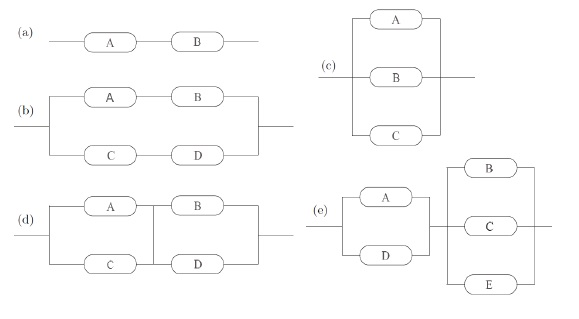
\includegraphics[width=1\linewidth]{uklady.jpg}
    \end{figure}
\end{zadanie}
\begin{proof}

    Niech kolejne pięć niezawodności będzie oznaczone jako: $P_A=0.9, P_B=0.8, P_C=0.7, P_D=0.6, P_E=0.5$. Umawiamy się również na konwencję zapisu $p' = 1-p$. Oczywiscie $p'' = p$. Wyznaczymy teraz następujące zasady rozwiązywania układów:

    \begin{itemize}
        \item Niezawodność zastępcza układów szeregowych jest iloczynem ich niezawodności: $P_{12} = P_1\cdot\P_2$.
        \item Niezawodność zastępcza układów równoległych jest dopełnieniem iloczynu dopełnień ich niezawodności: $P_{12} = (P_1'\cdot P_2')'$ (lub, zapisując inaczej, $P_{12}' = P_1'\cdot P_2'$).
    \end{itemize}

    Widzimy tutaj dużą analogię z układami oporów ze szkolnych zadań z układów elektrycznych - dodawanie oporów jest zastąpione mnożeniem, natomiast odwrotności oporów - dopełnieniami.

    \begin{enumerate}[a)]
        \item Układ działa, jeśli obydwa przekaźniki działają. Niezawodność układu będzie zatem iloczynem niezawodności obydwu przekaźników:

              $$P_{AB} = P_{A}\cdot P_{B} = 0.72.$$
        \item Układ działa, jeśli nie występuje przypadek jednoczesnego niedziałania dwóch podukładów. Zatem, niezawodność układu wynosi:

              $$P_{ABCD} = (P_{AB}'\cdot P_{CD}')' = ((P_AP_B)'(P_CP_D)')' = ((0.9\cdot 0.8)'(0.7\cdot 0.6)')' = 0.8376.$$

        \item Układ działa, jeśli przynajmniej jeden z podukładów działa:

              $$P_{ABC} = (P_A'\cdot P_B'\cdot P_C')' = 0.994.$$

        \item Układ działa, jeśli obydwa dwa podukłady działają:

              $$P_{ABCD} = (P_A'P_C')'\cdot(P_B'P_D')' = 0.8924.$$

        \item Układ działa, jeśli obydwa podukłady działają:

              $$P_{ABCDE} = (P_A'\cdot P_D')'\cdot(P_B'P_C'P_E')' = 0.9312.$$

    \end{enumerate}
\end{proof}

\end{document}
